%%%%%%%%%%%%%%%%%%%%%%%%%%%%%%%%%%%%%%%%%%%%%%%%%%%%%%%%%%%%%%%%%%%%%%
%%                     Stimulation
%%%%%%%%%%%%%%%%%%%%%%%%%%%%%%%%%%%%%%%%%%%%%%%%%%%%%%%%%%%%%%%%%%%%%%

\paragraph{Glyph: \glyph{Stimulation}}\label{sec:stimulation}
%\color{blue}

A stimulation affects \textbf{positively} the flux of a process represented by the target process. This stimulation can be for instance a catalysis or a positive allosteric regulation. Note that \glyph{catalysis} exists independently in SBGN, see \sect{catalysis}.

\begin{glyphDescription}
 \glyphSboTerm SBO:0000170 ! stimulation.
 \glyphOrigin Any \glyph{EPN} (\sect{EPNs}) or any logical operator (\sect{logic}).
 \glyphTarget Any \glyph{process node} (\sect{PNs}).
 \glyphEndPoint The target extremity of a \glyph{stimulation} carries an empty arrowhead.
 \end{glyphDescription}

\begin{figure}[H]
  \centering
  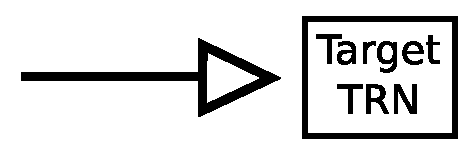
\includegraphics[scale = 0.5]{images/stimulation}
  \caption{The \PD glyph for \glyph{stimulation}.}
  \label{fig:stimulation}
\end{figure}


